\begin{figure*}[t]
\def\bb{\rule{2in}{0pt}\rule{0pt}{1in}}
\begin{center}
% \includegraphics[width=\linewidth,trim=0 170 70 0,clip ]{method/overview_v3.pdf}
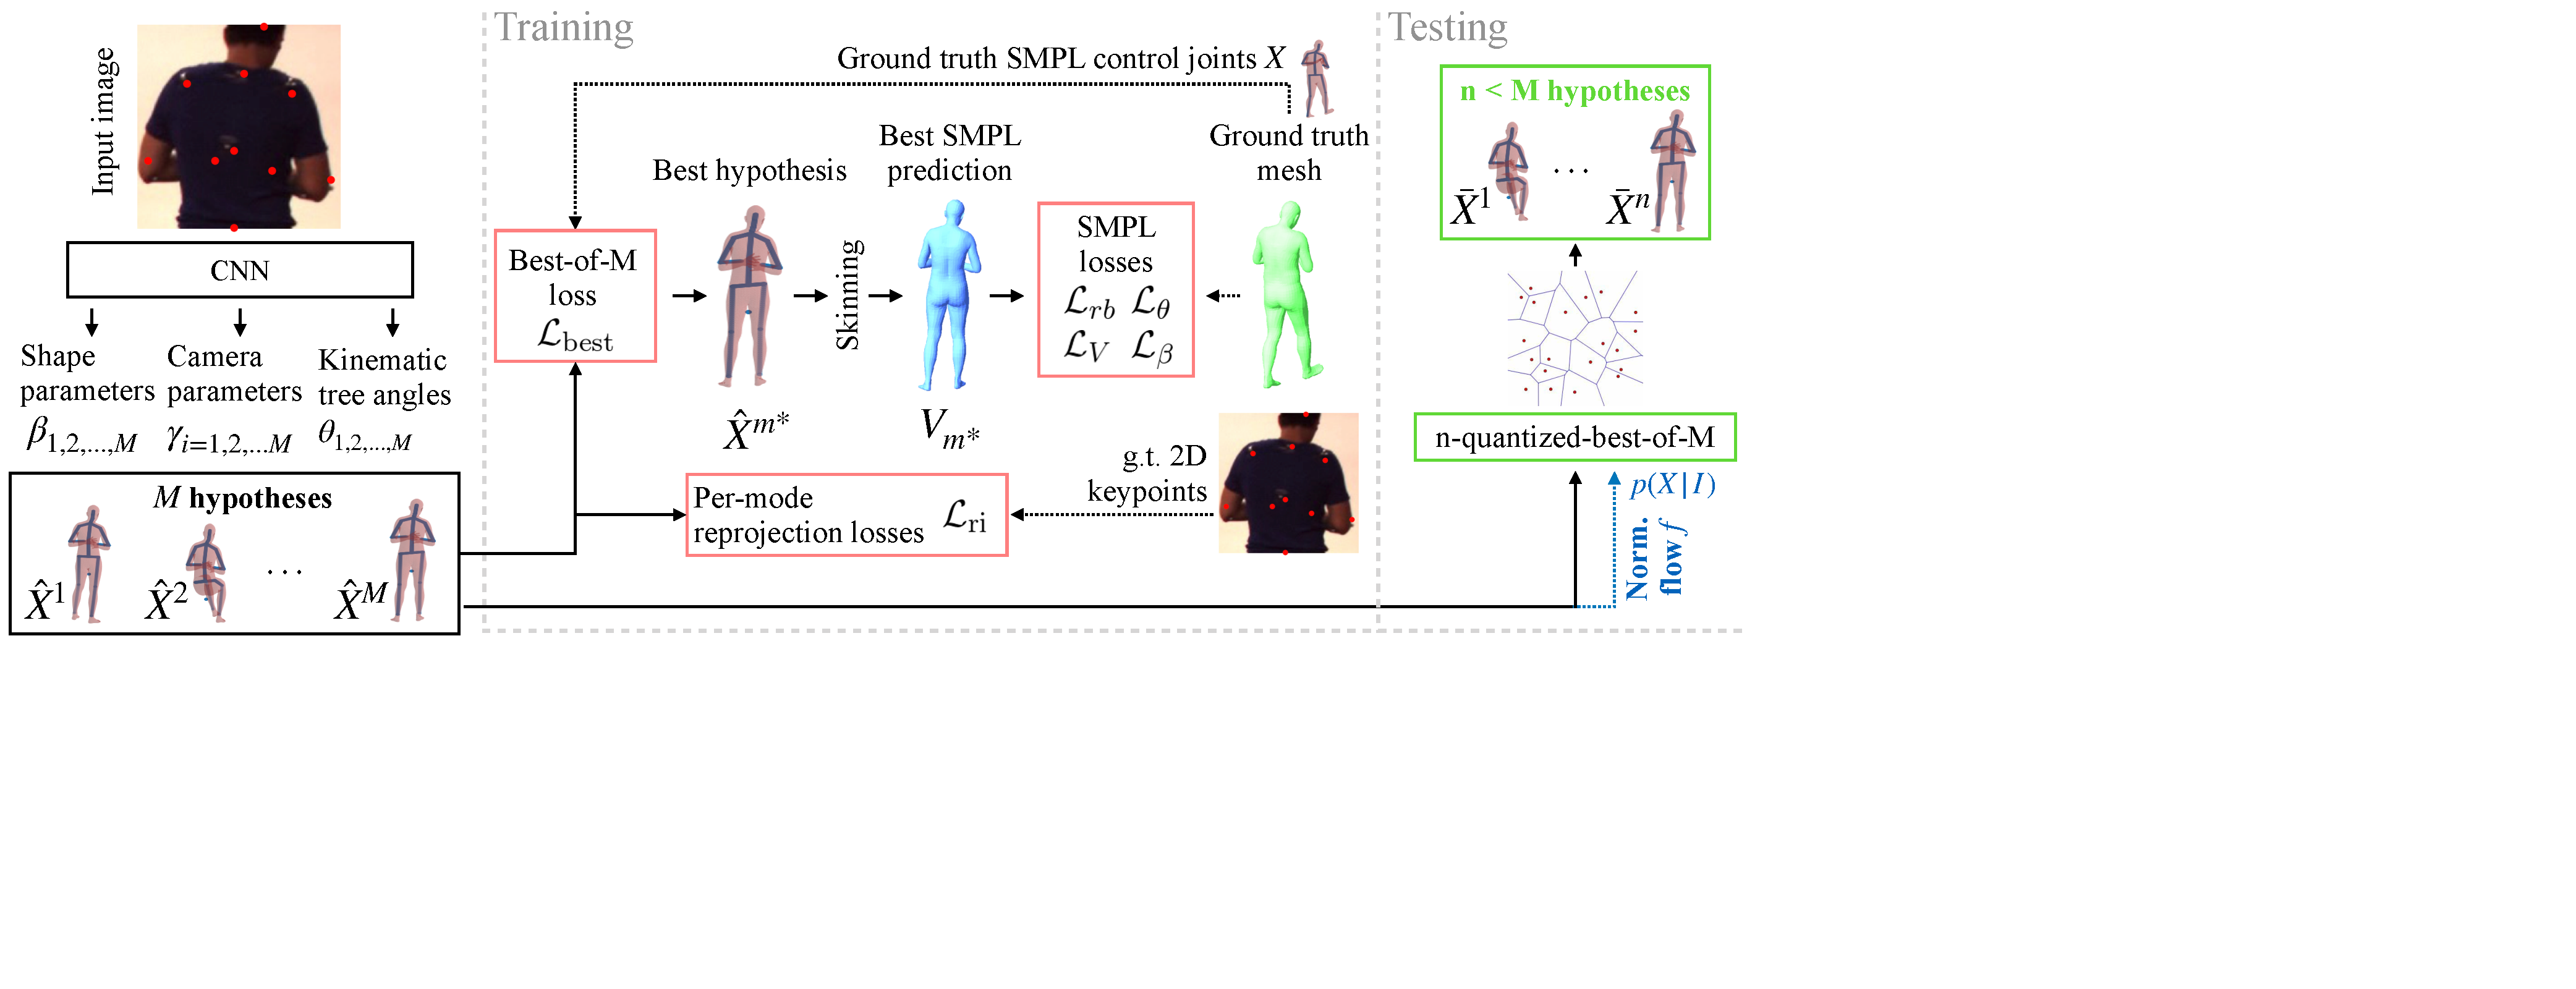
\includegraphics[width=\linewidth]{method/overview_v6.pdf}
\end{center}
\caption{\textbf{Overview of our method.}
Given a single image of a human, during training, our method produces multiple skeleton hypotheses $\{\hat X^i\}_{i=1}^M$ that enter a Best-of-$M$ loss which selects the representative $\hat X^{m^*}$ which most accurately matches the ground truth control joints $X$. 
% The camera parameters together with a skinned SMPL mesh enter the final set of SMPL losses.
At test time, we sample an arbitrary number of $n<M$ hypotheses by quantizing the set $\{\hat X^i\}$ that is assumed to be sampled from the probability distribution $p(X|I)$ modeled with normalizing flow $f$.
}\label{fig:arch_diagram}
\end{figure*}